\section{Softwarearchitektur}
\label{sec:Kap-7.1}

Die Softwarearchitektur beschreibt die Gesamtstruktur eines Softwaresystems. Sie stellt auf einer hohen Abstraktionsebene dar, aus welchen großen Komponenten das System aufgebaut sein soll, wie diese Komponenten zueinander in Beziehung stehen, auf welche Weise sie miteinander interagieren und wie das Gesamtsystem und seine Komponenten mit Elementen außerhalb des Systems interagieren.

\vspace{2mm} %%% für Druck

Eine Komponente ist grundsätzlich eine Einheit zusammengehöriger Funktionalität. \marginline{Komponente} Der Begriff Komponente wird im Rahmen des Softwareentwurfs für sehr unterschiedlich „große“ Teile des Softwareprodukts verwendet. Auf einer niedrigen Abstraktions\-ebene kann man eine Klasse als Komponente des Programms betrachten oder sogar eine Operation als Komponente einer Klasse. Aus der hohen Abstraktions\-sicht der Softwarearchitektur ist eine Komponente ein komplettes Teilstück des Software\-produkts, wie zum Beispiel die Benutzungsschnittstelle, die Datenhaltung, ein Authentifizierungs- oder ein Logging-Mechanismus, das selbst wieder aus kleineren Komponenten zusammengesetzt sein kann.

\vspace{2mm} %%% für Druck

Der Entwurf der Architektur des Softwaresystems ist in der Regel der erste Schritt im Prozess des Softwareentwurfs. Will man die Architektur im späteren Verlauf des Softwareentwicklungsprojekts überarbeiten, ist das meistens teuer, da man sehr viele schon spezifizierte oder sogar schon umgesetzte einzelne Komponenten verändern muss. Eventuell muss man sogar von vorne beginnen.

\vspace{2mm} %%% für Druck

Die für ein Softwaresystem gewählte Architektur hat einen grundlegenden Einfluss darauf, wie sich das System im späteren Einsatz verhält. Ungünstig getroffene architektonische Entscheidungen können Konsequenzen haben, die man schlimmstenfalls erst beim späteren Betrieb des Softwareprodukts bemerkt. Abbildung~\ref{fig:einfluss_architekturentscheidung} zeigt ein eingängiges – wenn auch IT-fernes – Beispiel aus \cite[97]{som20}, bei dem sich eine Architekturentscheidung auf die Systemsicherheit ausgewirkt hat.

\vspace{2mm} %%% für Druck

\begin{figure}[h!]
	\centering
	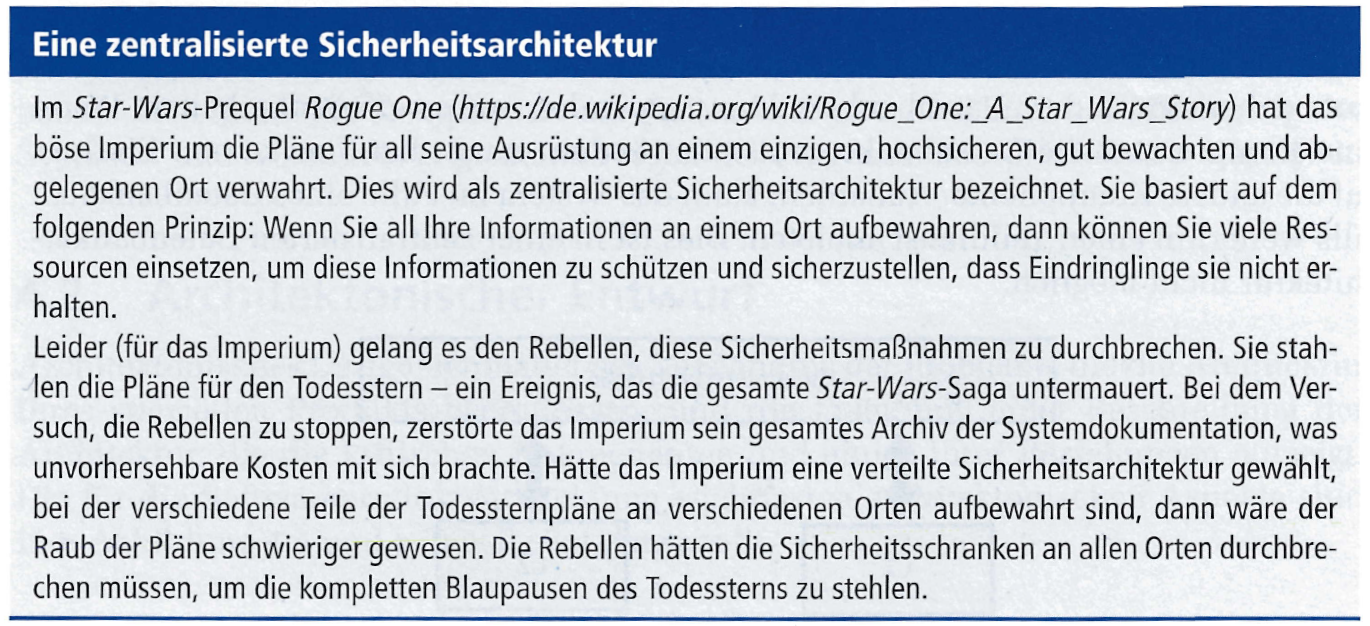
\includegraphics[width=\textwidth]{Bilder/Kapitel-7/einfluss_architekturentscheidung.png}
	\caption[IT-fernes Beispiel für den Einfluss einer Architekturentscheidung auf die Systemeigenschaften]{IT-fernes Beispiel für den Einfluss einer Architekturentscheidung auf die Systemeigenschaften \cite[97]{som20}}
	\label{fig:einfluss_architekturentscheidung}
\end{figure}

\minisec{Architekturen dokumentieren}

Über spezifische Architekturbeschreibungssprachen kann eine Softwarearchitektur sehr formal und sehr detailliert modelliert werden. Auch die UML bietet Diagramme (Komponentendiagramm, Verteilungsdiagramm, eingeschränkt auch Paket-
\linebreak %%% für Druck
diagramm) zur Modellierung der Softwarearchitektur an. Häufig arbeitet man in der Praxis aber mit sehr informellen Diagrammen, zum Beispiel indem Komponenten einfach als (auch ineinander geschachtelte) Kästen gezeichnet und mit Pfeilen zwischen ihnen grob die Beziehungen dargestellt werden. Gerade während der Entstehungszeit der Softwarearchitektur, wenn noch viel mündlich diskutiert wird und Anpassungen vorgenommen werden, ist ein solches informelles Vorgehen sinnvoll, weil es deutlich weniger aufwändig ist. Die Erstellung einer endgültigen „schriftlichen“ Architekturspezifikation als Basis für die Implementierung – manche Projekte verzichten allerdings darauf – oder die Dokumentation einer vorhandenen Architektur erfordert detailliertere Ausdrucksmöglichkeiten als einfache Kästen und Pfeile. Für solche Zwecke muss dann die UML oder eine spezifische Architekturbeschreibungssprache verwendet werden. Dies erfordert die Einarbeitung aller Beteiligten in die gewählte Sprache. Vor allem in agilen Projekten bleibt es zwar häufig bei den informellen Beschreibungen statt einer detaillierteren Ausarbeitung. Die grundsätzlichen Entscheidungen zur Softwarearchitektur müssen allerdings auch dort getroffen werden, auch agile Projekte kommen nicht ohne Architekturentwurf aus.